\chapter{Background and Related Work}
\label{ch:background}

    \section{Monitoring}
    \label{sec:monitoring-background}

        Monitoring is the process of continuously observing and tracking a system, process, or activity in order to gather data, identify trends, and detect any deviations or issues.
        Monitoring has the purpose of ensuring that the system is functioning as intended and also identifying any potential problems early on in order to mitigate them. Additionally, monitoring provides necessary information for effective decision-making and problem-solving.
        There are different monitoring types, including \emph{system-, environmental-, process-, performance- and security monitoring}.
        We mainly focus on \textbf{system monitoring}.
        Monitoring can be performed manually or through the use of automated tools and technologies.
        The choice of monitoring approach will depend on the specific requirements of the system or process being monitored.

        System monitoring involves monitoring the performance and availability of computer systems, applications and networks.
        This includes monitoring CPU, server memory, routers, switches, bandwidth, and applications as well as the performance and availability of important network devices. 
        These systems are also used to track information regarding items such as free disk space on available hard drives, and the temperature of hardware components such as the CPU.
        The advantage of using system monitoring is that in case of an occurring error or failure of a system component, the monitoring system will immediately send a notification and in the best case be able to fix the problem.
        Additionally, collecting data when a problem occurs also enables continuous improvement and easier debugging of faulty components.



        % \subsection{Process Monitoring}
        % \label{sec:process-monitoring-background}

        %     Process monitoring involves monitoring industrial processes to ensure they are operating efficiently and safely.




    \section{Computing Continuum}
    \label{sec:computing-continuum-background}

        Placeholder


    \section{Scheduling and Adaptation}
    \label{sec:scheduling-and-adaptation-background}

        \subsection{Adaptation}
        The SAA adaptation approach is defined as a loop, that cyclically updates every component contained in the loop.
        The adaptation loop is shown in figure \ref{fig:adaptation-loop} and consists of the Big Data pipeline and the \emph{resources} containing all registered and monitored to the \emph{Monitoring and Analysis} component. 
        Both the Big Data pipeline and the resources send the gathered monitoring information at a time step $P_t$ or $S_t$ respectively to the \emph{Monitoring and Analysis} component, where $t$ denotes the current time step.

        The Monitoring and Analysis component then uses the monitoring data $P_t$ and $S_t$ and calculates an action $A_{t+1}$ as an update for the resources, where $t+1$ denotes the next time step.
  
        This received action $A_{t+1}$ is then used by the Resource components to reconfigure the resources if necessary.
        The adaptation uses monitoring of tasks and resources to retrieve the monitoring data $P_t$, $S_t$.
        
        The monitoring component is necessary to obtain information about failures or performance fluctuations along with under-, and over-utilisation of resources.
        The monitoring data, therefore, provide feedback if a resource can handle the additional load, and thus, more tasks will potentially be mapped to it for execution. 
        In case the resource is not capable of handling the current load, less demanding tasks will be mapped to that resource in future scheduling cycles and it will be reconfigured accordingly.

        A monitored resource information consists of the CPU, memory and storage utilization, in addition to network bandwidth usage.
        The Big Data pipeline and resources send their monitoring data $P_t$, and $S_t$ respectively to the Monitoring and Analysis component.
        Afterwards, given those monitoring data, the analyser will determine the next action $A_{t+1}$ of the resources.
        The monitoring feedback will be periodically retrieved from all registered resources and provided to the analyser.
        In case of a resource side failure, the monitoring mechanism will be alerted of the occurred anomaly.  
        The analyser uses this monitoring data to decide if any actions $a \in A$ on the current scheduling plan have to be applied.
  
        \begin{figure}[h!]
            \centering
            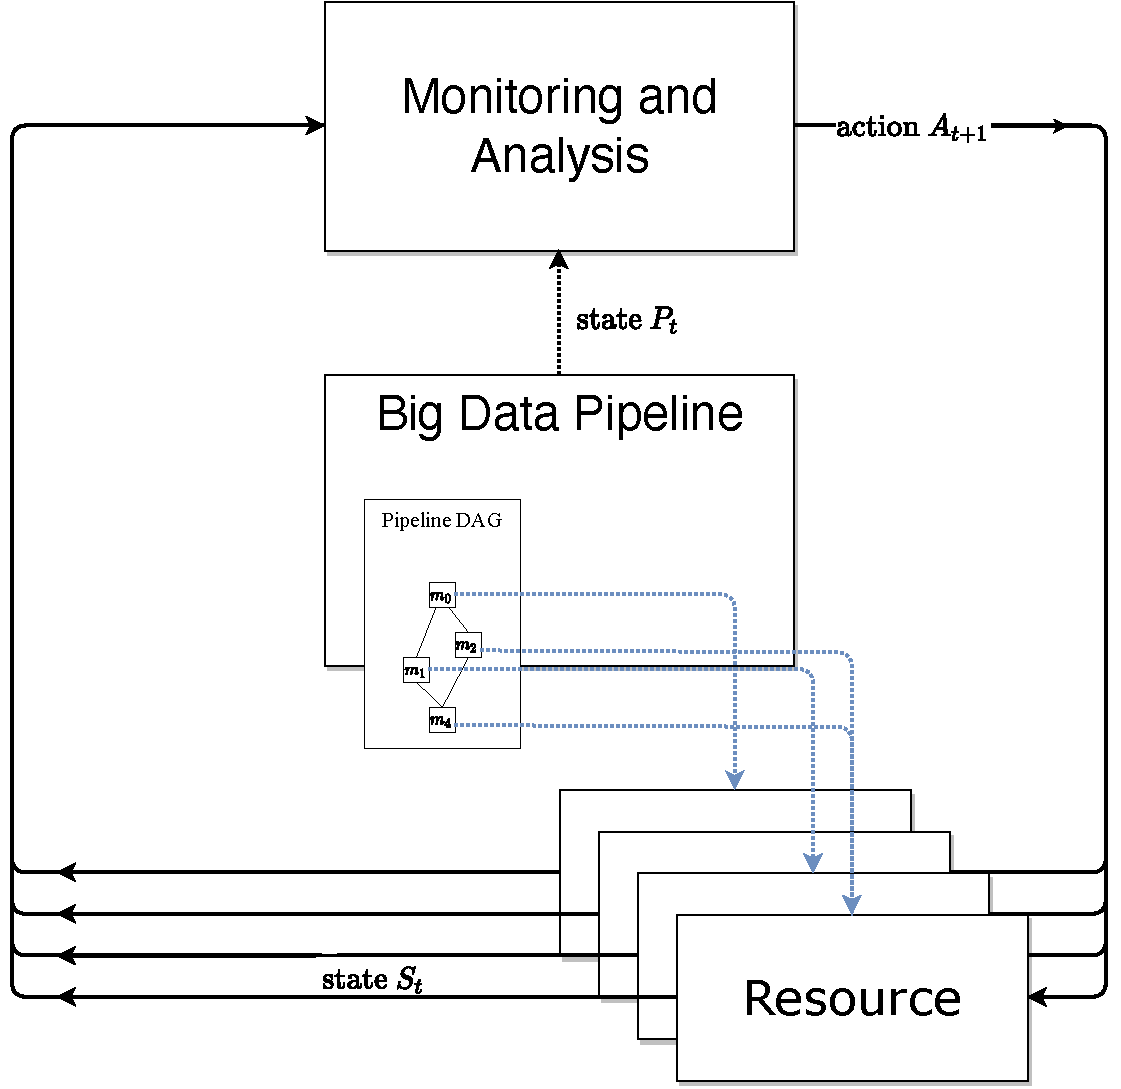
\includegraphics[width=\columnwidth]{figures/monitoring_with_inner_resources.drawio.pdf}
            \caption{Adaptation Loop}
            \label{fig:adaptation-loop}
        \end{figure}
        The following actions $A$ are considered in the adaptation approach:

        \subsubsection*{Resource load within expected parameters $(S_1)$} 
        When tasks on resources are well mapped and no action has to be taken for these resources, this is denoted in the action set $A_{t+1}$ as the state $S_1$. This state is achieved when a resource is running within expected parameters, the estimated time of completing a task is not exceeded or other anomalies occur.

        \subsubsection*{Resource load under expected parameters $(S_2)$} 
        When the monitoring component detects under-utilization of a resource, tasks of the pipeline are mapped to it to be efficiently utilized. This state is categorized as $S_2$ in the analyser and the action set will be modified to improve the utilization of resources grouped into $S_2$. 

        \subsubsection*{Resource load over expected parameters $(S_3)$} 
        If a resource is over-utilized, there are multiple options. If it is detected that horizontal scaling solves the over-utilization and the resource instance is capable of being scaled up, it will be reconfigured to be within expected utilization levels. Furthermore, if an ill-defined task is detected and was mapped to a resource that isn't capable to fulfil the computation within a reasonable time frame, this task will be migrated to another resource. 
        This is categorized as $S_3$ in the analyser, and the action set will be modified, so that resources grouped in $S_3$ will be less utilized with the upcoming updates of the action set.

    \subsection{Scheduling and Adaptation Functional Architecture}
        The architecture of the integrated \SAA{} scheduling and adaptation tool consists of five components, displayed in Figure~\ref{fig:data-cloud-architecture}.

        \begin{figure}
            \centering
            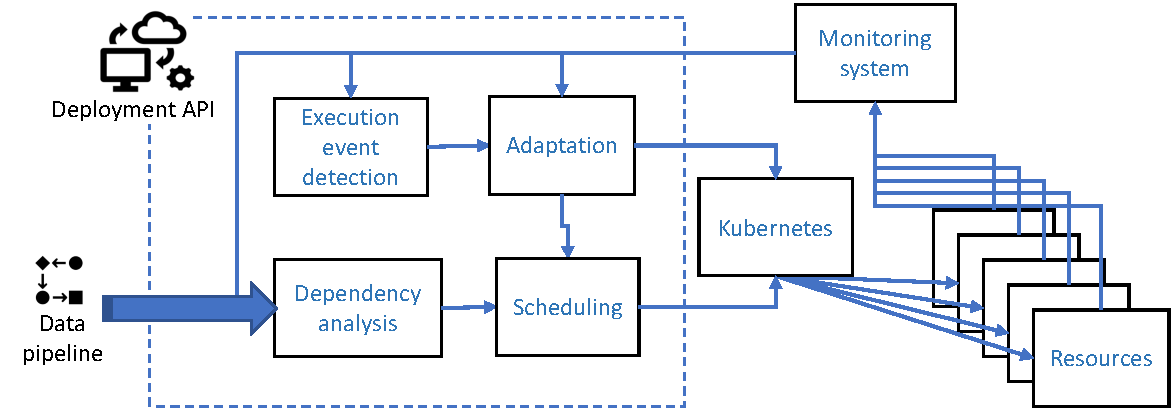
\includegraphics[width=0.8\textwidth]{pdf/data_cloud_arch.pdf}
            \caption{\SAA Architecture}
            \label{fig:data-cloud-architecture}
        \end{figure}

        \paragraph{Dependency analysis } orders the candidate tasks scheduled on each resource in a preference list based on the aggregate pipeline communication time to each task.

        \paragraph{Execution event detection } uses data from external monitoring system to identify SLO violations or anomalies during execution.

        \paragraph{Scheduling } maps the pipeline tasks to the resources using a matching theory algorithm, applied on the task and resource preference lists in response to infrastructure drifts.

        \paragraph{Adaptation } dynamical applies re-scheduling or migration of the tasks based on the analyzed monitoring received from the execution event detection. Both the scheduling and adaptation interact with deployment and orchestration system to perform deployment and adaptation of the tasks.

        \paragraph{Public API } enables the integration of the \SAA{} scheduling and adaptation tool with deployment and orchestration systems. \cite{kimovskiBigDataPipeline2022}

    \section{Prediction of Load}
    \label{sec:prediction-of-load-background}

        User-based prediction via domain expertise

    \section{Supervised Learning}
    \label{sec:supervised-learning}

        Supervised learning is a machine learning paradigm that is applied when available data consists of labelled data points, that not only contain features but also a label that is associated with these features.
        Supervised learning is defined by its use of labelled datasets to train algorithms to classify data or predict outcomes accurately.
        As input data is fed into the model, it adjusts its weights until the model has been fitted appropriately, which occurs as part of the cross-validation process.
        Supervised Learning uses a training set to teach models to yield the desired output.  
        This training dataset includes inputs and correct outputs, which allow the model to learn over time. The algorithm measures its accuracy through a loss function, adjusting until the error rate has been sufficiently minimized.
        A training dataset with $n$ are of the form $\left\{(x_1, y_1), \dots , (x_n, y_n)\right\}$ such that $x_i$ is defined as the \emph{feature vector} of the $i$-th data point and $y_i$ is defined as its label.
        A supervised learning algorithm will train to learn a function $g$ such that $g: X \rightarrow Y$, where $X$ is the input space and $Y$ is the output space.
        The function $g$ is often represented as a scoring function $f: X \times Y \rightarrow \mathcal{R}$ such that $g$ is defined as $g(x) = \arg \max f(x, y)$ such that $g$ returns the $y$ value with the highest score.
        Supervised learning can be separated into \nameref{sec:classification-supervised-learning-background} and \nameref{sec:regression-supervised-learning-background} problems.

        In supervised learning for scheduling the objective is to learn parameters of the neural network such that the trained networks can replicate the behaviour of pre-existing scheduling methods, such as mathematical optimisations, and search methods, for example \emph{Priority Dispatching Rule (PDR)}, a heuristic rule that assigns jobs to machines based on their priorities while considering the current status of the system.
        Supervised learning can also be used for forecast models that predict the resource utilisation or the runtime of tasks.
        This is done by providing information such as the capacity of a resource, the naive allocation prediction provided by a human and other factors to the feature vector and including the target that is to be predicted to the labels. 
        The training dataset for this prediction task is usually a time series forecasting dataset.
        In a time series forecasting dataset, the order of data points is ascending, meaning that the structure and order of the data points is used as additional information that is used for the prediction.

        \subsection{Classification}
        \label{sec:classification-supervised-learning-background}

            A classification problem is when the output value is a categorical data type, such as "cat" and "dog".
            This section is added for completeness but won't be discussed further since it serves no purpose for this masters thesis.

        \subsection{Regression}
        \label{sec:regression-supervised-learning-background}

            Regression is used to predict continuous-valued outputs. That is, find a relationship between the input and output data generated by an unknown but fixed distribution represented by a function denoted as $f(x)$. 
            A regression model does so by showing whether the observed changes in the dependent variable are also associated with changes in the independent (explanatory) variables. 
            \begin{figure}[h!]
                \centering
                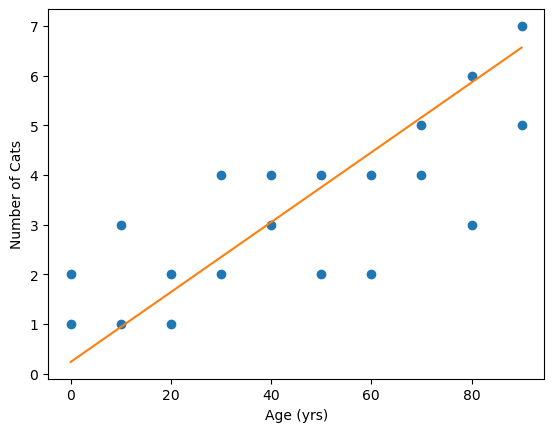
\includegraphics[scale=0.6]{figures/regression_plot.png}
                \caption{Regression Example}
                \label{fig:regression-example}
            \end{figure}
            In figure \ref{fig:regression-example} an example regression is shown by the orange line that is done by linear regression. As can be seen, the linear regression line is estimating the values of the data points by trying to fit closest to all data points that are shown as the blue dots.
            This is done by using the function $f(x)$ to find a best-fit line and see how much the data is dispersed around this line.
            \begin{quote}
                Regression is a statistical method used in finance, investing, and other disciplines that attempt to determine the strength and character of the relationship between one dependent variable (usually denoted by Y) and a series of other variables (known as independent variables). \cite{beersWhatRegressionDefinition}
            \end{quote}
            Therefore, regression analysis is a useful tool for finding associations of variables that are observed in data. Yet, those associations do not indicate causation but merely correlation.
            This is because regression only captures correlations between variables that are observed in data and quantifies if the found correlation is statistically significant.
            In order for proper interpretations regarding the regression results, several assumptions about the data and the model itself must hold.

    \section{Recurrent Neural Network}
    \label{sec:rnn-background}

        Recurrent Neural Networks (RNNs) are a type of neural network designed to handle sequential data.
        Opposed to traditional feedforward neural networks, which receive a fixed-sized vector as input and produce a fixed-sized vector as output, 
        RNNs are able to handle sequences of variable length and produce a hidden state that summarizes information from the entire sequence.
        \begin{figure}[h!]
            \centering
            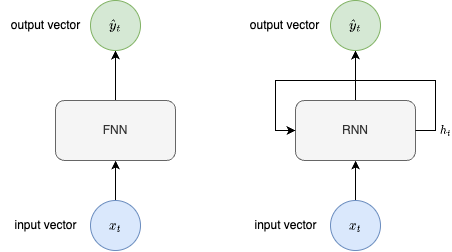
\includegraphics[scale=0.5]{figures/FNN_vs_RNN.drawio.png}
            \caption{FNN vs. RNN}
            \label{fig:fnn-vs-rnn}
        \end{figure}
        In an RNN, each unit in the network processes the input sequence one-time step at a time, maintaining a hidden state that summarizes information from all previous time steps. At each time step, the hidden state is updated based on both the current input and the hidden state from the previous time step. The hidden state is then used to generate the output for that time step, and the process is repeated for each time step in the sequence.
        RNNs are used for a variety of tasks, including natural language processing, speech recognition, and video analysis. They can also be used to generate sequences, such as in text generation or music composition.


        The ability to maintain information across a sequence of inputs makes RNNs a fitting tool for modelling sequential data.
        \begin{quote}
            ... recurrent neural networks contain cycles that feed the network activations from a previous time step as inputs to the network to influence predictions at the current time step. These activations are stored in the internal states of the network which can in principle hold long-term temporal contextual information. This mechanism allows RNNs to exploit a dynamically changing contextual window over the input sequence history. \cite{sakLongShortTermMemory2014}
        \end{quote}
        Yet, this also results in them being prone to \nameref{par:vanishing-gradients-background} and \nameref{par:exploding-gradients-background}, which make it cumbersome to train the network effectively. 
        To address these issues, several variants of RNNs have been developed, \nameref{sec:lstm-background} networks and Gated Recurrent Units (GRUs).
        
        
        \subsection{Recurrent Cell Architecture}
        \label{sec:recurrent-cell-architecture-background}

            A traditional feed-forward neural network (FNN) is unidirectional, meaning that they have a single direction and hence cannot persist information over a time step $t$.
            Looping structures are added to a feed-forward neural network that enables the persistence of information about time-series or sequential data. 
            This is the reason RNNs are known as "recurrent" neural networks.

            As can be seen in figure \ref{fig:fnn-vs-rnn}, the RNN has an additional loop inside it to persist time-series information. The loop structure enables the RNN to apply a \emph{recurrence relation} (see \ref{sec:recurrence-relation-background}) at every time step in order to process a sequence.

            The rectangle containing the "RNN" label is defined as a "recurrent cell".
            This workflow of a single RNN cell can be seen in more detail in figure \ref{fig:single-rnn-cell}, where the previous cell state $h_{t-1}$ and the current input $x_t$ are used as the input of the recurrent cell, get combined and forwarded to the $tanh$ \emph{activation function}, which returns the output vector $\hat{y}_t$ and $h_t$ (the recurrence relation).

        \subsection{Recurrence Relation}
        \label{sec:recurrence-relation-background}

            The recurrence relation is applied at every time step to process a sequence.

            The recurrent relation seen in figures \ref{fig:fnn-vs-rnn}, \ref{fig:single-rnn-cell} is denoted as $h_t$ and is defined as $h_t = f_w(h_{t - 1}, x_t)$, where $f_w$ is a function that is parametrized by the weights, $h_{t-1}$ is the previous state and $x_t$ is the input vector at time step $t$. With the addition of $h_{t-1}$, the model is now also taking the previous time step into account when updating the current time step. 
            \begin{figure}[h!]
                \centering
                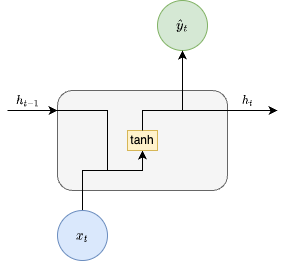
\includegraphics[scale=0.5]{figures/single_rnn_cell.drawio.png}
                \caption{Single RNN Cell}
                \label{fig:single-rnn-cell}
            \end{figure}

            
            \begin{pabox}{Recurrence Relation}
                \label{def:lstm-recurrence-relation-definition}
                The recurrence relation in a more mathematical notation is:
                $$h_t = \tanh(W^T_{hh} h_{t-1} + W^T_{xh} x_t)$$
                Both the input vector $x_t$ as well as the previous state $h_{t-1}$ are multiplied with the two separate weight matrices $W^T_{xh}$ and $W^T{hh}$ respectively, combined and fed to the $\tanh$ activation function. Finally, the $\tanh$ function returns the output vector $\hat{y}_t$ at time step $t$.
            \end{pabox}
            

        \subsection{RNN Loop Unfolding}
        \label{sec:rnn-loop-unfolding-background}

            The loop unfolding will provide a description about how RNN handles sequential data at every time step.
            As can be seen in figure \ref{fig:rnn-loop-unfolding}, the model is adding the input at every time step, and generates an output $\hat{y}_i$ for every time step.
            The weight matrices $W_{hh}$ that are used for every time step for updating the previous state are the same for every time step.
            The weight matrix $W_{xh}$ is applied to every $x_i$ and is also the same for every time step $i$.

            \begin{figure}[h!]
                \centering
                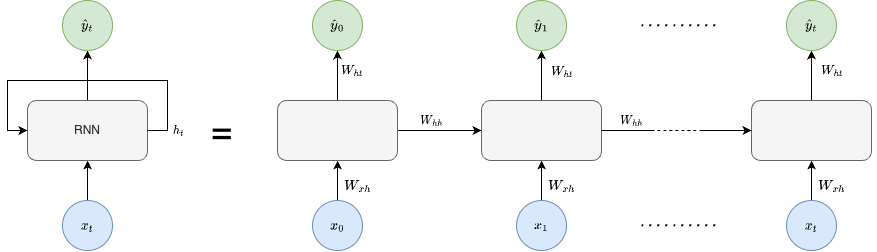
\includegraphics[width=0.90\textwidth]{figures/rnn_loop_unfolding.drawio.png}
                \caption{RNN Loop Unfolding}
                \label{fig:rnn-loop-unfolding}
            \end{figure}
            \begin{itemize}[label=\textemdash]
                \item $x_i$ denotes the input value at time step $i$.
                \item $\hat{y}_i$ denotes the output value at time step $i$.
                \item $W_{hh}$ denotes the weight matrix to update the previous state.
                \item $W_{xh}$ denotes the weight matrix that is applied to the input value at every time step.
            \end{itemize}
            The output vectors $\hat{y}_0, \hat{y}_1, \hat{y}_2, \dots, \hat{y}_t$ can be used to calculate the separate losses $L_0, L_1, L_2, \dots, L_t$ at each time step $t$.
            % This completes the forward propagation (see \ref{sec:forward-propagation}).

        \subsection{Loss Calculation and Weight Updates for RNN}
        \label{sec:loss-calculation-and-weight-updates-for-rnn-background}
        
            The training of an unfolded RNN is done through multiple time steps, as can be seen in figure \ref{fig:rnn-loop-unfolding}.
            The overall loss is defined as $L = L_0, L_1, \dots, L_t$ and is calculated from the outputs $\hat{y}_0, \hat{y}_1, \dots, \hat{y}_t$  for each time step $t$ in the \emph{forward-propagation} process.
            \begin{figure}[h!]
                \centering
                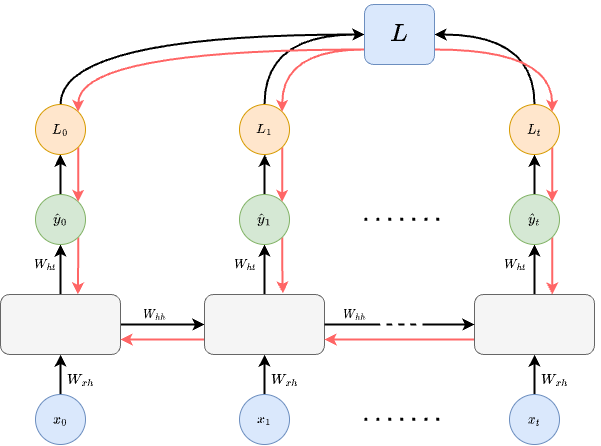
\includegraphics[width=0.6\textwidth]{figures/rnn_loss_calculation.drawio.png}
                \caption{Loss Calculation and Weight Update in RNNs}
                \label{fig:loss-calculation-weight-update-rnn}
            \end{figure}
            Then the total loss $L$ is used to propagate backwards and calculate the \emph{back-propagation} in order to update the weights of the model.
            This is shown in figure \ref{fig:loss-calculation-weight-update-rnn}, where the black arrows display the forward-propagation step that is accumulated as the total loss $L$, and then the back-propagation shown as the red arrows update the weights by using the partial derivative.

            \begin{quote}
                The central problem that back-propagation solves is the evaluation of the influence of a parameter on a function whose computation involves several elementary \emph{steps}. The solution to this problem is given by the chain rule, but back-propagation exploits the particular form of the functions used at each step (or layer) to provide an elegant and local procedure. \cite{lecunTheoreticalFrameworkBackpropagation1988}
            \end{quote}
            Backpropagation is the practice of fine-tuning the weights of a neural network based on the error rate (i.e. loss) obtained in the previous epoch. Proper tuning of the weights ensures lower error rates, making the model reliable by increasing its generalization.


        \subsection{Common Problems and Shortcomings of RNNs}
        \label{sec:shortcomings-of-rnns-background}

            Regularly experienced problems of RNNs are the exploding or vanishing gradient problems.
            \begin{quote}
                The motivation behind why they happen is that it is hard to catch long-haul conditions as a result of a multiplicative angle that can be dramatically diminishing/expanding regarding the number of layers. \cite{parikhDisadvantagesRNN2021}
            \end{quote}
            While unfolding, the error gradient is calculated as the sum of all gradient errors across time steps. Therefore, the loss calculation in unfolded RNNs is also known as \emph{backpropagation through time (BPTT)}.
            Over time while calculating the error gradients the domination of the multiplicative term increases due to the chain rule application. And thus the gradients either explode or vanish.
            These problems occur when the sequence is too long and this may result in the model training with either null weights (i.e. the model won't learn while training) or exploding weights.
            
            \paragraph{Exploding Gradients}
            \label{par:exploding-gradients-background}

                The Exploding Gradients problem occurs when many of the values (i.e. weight matrices, or gradients themselves) involved in the repeated gradient computations are greater than 1. 
                If this is the case, then gradients become extremely large and optimising them becomes computationally intensive.
                To solve the Exploding Gradients problem, a process called \emph{Gradient Clipping} is applied, which scales the gradient values to smaller values less than 1.


            \paragraph{Vanishing Gradients}
            \label{par:vanishing-gradients-background}

                The Vanishing Gradients problem occurs when many of the values (i.e. weight matrices or gradients themselves) that are involved in the repeated gradient computations are too small or less than 1. Opposed to the \nameref{par:exploding-gradients-background} problem, the gradients become smaller with each repeated computation of the gradients.
                This results in the problem of \emph{long term dependency}, where smaller sequences can be remembered and the weights updated accordingly. But for longer sequences, the model will unlikely be able to yield a good prediction performance.

                There are multiple solutions to the Vanishing Gradient problem, such as changing the activation function from $\tanh$ to \emph{Rectified Linear Unit (ReLU)}. Also initialising the weights of the model can solve this problem, though tailored heuristics (such as the \emph{Xavier Weight Initialisation}) should be used to result in omitting the Vanishing Gradients problem and also increase the efficiency of the training. Another solution is to change the architecture of the neural network and add more complex recurrent units that are mentioned in section \ref{sec:lstm-background}.

            \paragraph{Slow and Complex Training}

                Since RNNs are recurrent one of their fundamental problems is that they require a lot of time for training when compared to FNNs. Additionally, RNNs need to calibrate the previous outputs as well as current inputs into a state change function, which in turn makes RNNs harder to implement and customize and more complex to train.

            \paragraph{Difficult to Process Longer Sequences}

                As already mentioned earlier, training RNNs on too-long sequences is difficult without taking any measures to improve the prediction performance. This is especially true while using the $tanh$ activation function. 
                
    \section{Long-Short Term Memory}
    \label{sec:lstm-background}

        \emph{Long-Short Term Memory (LSTM)} \cite{hochreiterLongShortTermMemory1997} \cite{gravesLongShorttermMemory2012} are a type of \nameref{sec:rnn-background} architecture but are designed to improve upon the issues of regular RNN models as are mentioned in \nameref{par:vanishing-gradients-background} and \nameref{par:exploding-gradients-background}. 
        The main architectural improvement for LSTMs over traditional RNNs is that they have introduced \nameref{sec:lstm-memory-cell-architecture-background} to produce paths, which let gradients flow for a long duration, and thus gradients will not vanish.
        Compared to RNNs, LSTMs are better suited for learning long-term dependencies in sequential or time-series data that have temporal dependence such as natural language processing, speech recognition, music generation and financial prediction.
        \begin{quote}
            Hence standard RNNs fail to learn in the presence of time lags greater than 5 – 10 discrete time steps between relevant input events and target signals. The vanishing error problem casts doubt on whether standard RNNs can indeed exhibit significant practical advantages over time window-based feedforward networks. A recent model, “Long Short-Term Memory” (LSTM), is not affected by this problem. LSTM can learn to bridge minimal time lags in excess of 1000 discrete time steps by enforcing constant error flow through “constant error carousels” (CECs) within special units, called cells. \cite{gersLearningForgetContinual2000}
        \end{quote}
        LSTMs are a type of deep learning algorithm that can be trained end-to-end, making them highly flexible and suitable for complex problems where the underlying relationships between input and output are not well understood.



        \subsection{LSTM Memory Cell Architecture}
        \label{sec:lstm-memory-cell-architecture-background}

            The LSTM architecture is comprised of a series of memory cells that store information and gate mechanisms that are used to control the flow of information into and out of the cells.
            Compared to RNN cells, they are more complex and require more computations in general.
            The introduction of \emph{self-looping} to produce paths is the main architectural improvement for LSTMs over RNNs. This additional component diminishes the problem of the vanishing gradients problem and enables gradients to flow for a long duration when extended with gate units as is described in the upcoming sections.
            \begin{figure}[h!]
                \centering
                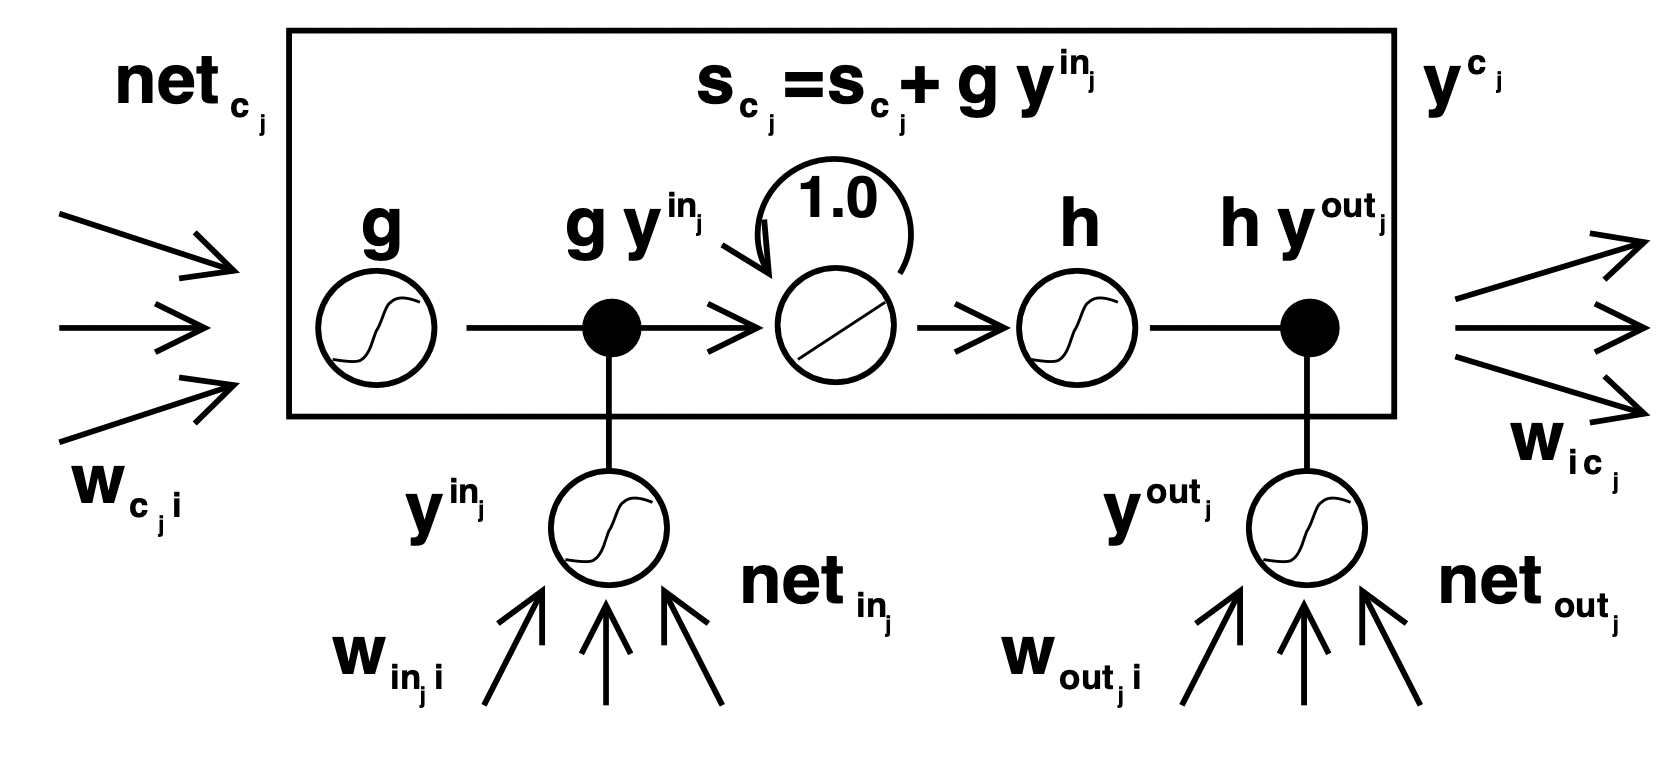
\includegraphics[width=0.6\textwidth]{figures/lstm_memory_cell.png}
                \caption{Architecture of a memory cell and its gate units \cite{hochreiterLongShortTermMemory1997}}
                \label{fig:architecture-of-a-memory-cell}
            \end{figure}
            LSTM memory cells can store information for an extended period compared to regular RNNs and its \emph{cell state} functions as the memory of the network.
            The architecture of a memory cell and its gates can be seen in figure \ref{fig:architecture-of-a-memory-cell} that was taken directly from the paper \cite{hochreiterLongShortTermMemory1997}.


            \subsubsection{LSTM Gate Structure}
            \label{sec:lstm-gate-structure}

                The key building block in LSTM cells is a gate structure.
                Each memory cell has gate components that control the flow of information into and out of the cell.
                Information is either added or removed through these gates.
                The usage of gates to control the information flow allows the LSTM model to selectively remember or forget information, making it well-suited for tasks that require long-term memory.
                The gate types are as follows:

            \subsubsection{Input Gate} 
            
                This gate determines the flow of new information and how much from the current time step should be added to the cell state. The input gate is implemented as a multiplicative gate that protects other units such as the cell state from perturbation by irrelevant input information.

            \subsubsection{Forget Gate}

                This gate determines how much of the previously obtained information should be forgotten in order for the network to maintain a long-term memory of relevant information and discard irrelevant information.
                \begin{pabox}{Forget Gate}
                    \label{def:lstm-forget-gate-definition}
                    The forget gate is denoted by $$f_i^{(t)} = \sigma \left(b_i^f + \sum_{j} U_{i, j}^f x_j^{(t)} + \sum_{j} W_{i, j}^f h_j^{(t - 1)}\right)$$ where $t$ is the time step and $i$ is the memory cell, $x^{(t)}$ is the current input vector, $h^{t}$ is the current hidden state containing the outputs of all the LSTM cells, $b^f$ is the bias, $U^f$ the input weights and $W^f$ the recurrent weights for the forget gates.
                \end{pabox}
                
                % which sets the weight value of the forget gate between $0$ and $1$. 

                

            \subsubsection{Output Gate}

                The output gate controls what information is being used for the cell state, and is sent to the network as input for the next time step. The output of the output gate is referred to as the \emph{hidden state}, denoted as $h_i^{(t)}$ and is sent to the next network layer or also used for predictions.



            \subsubsection{Sigmoid Layer and Pointwise-Multiplication}
            \label{sec:sigmoid-layer-and-pointwise-multiplication}

                Optionally, information can also be passed through by those gates via a Sigmoid layer and point-wise multiplication as can be seen in figure \ref{fig:sigmoid-layer-and-pointwise-multiplication}.
                \begin{figure}[h!]
                    \centering
                    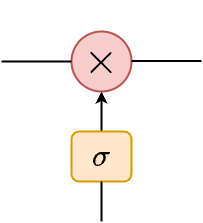
\includegraphics[width=0.2\textwidth]{figures/sigmoid_layer.drawio.png}
                    \caption{Sigmoid Layer and Pointwise Multiplication}
                    \label{fig:sigmoid-layer-and-pointwise-multiplication}
                \end{figure}
                The Sigmoid layer is used to map the input to an output in a range of $0$ and $1$, which is used to determine how much of the information is captured while passing through the gate, and how much of the information will be retained while the pass-through.
                If the Sigmoid output is $0$, no information is kept and if the Sigmoid output is $1$, all information about the input is kept.

            \subsubsection{Back-Propagation Through Time}
            \label{sec:back-propagation-through-time}

                The LSTM architecture implements so-called \emph{backpropagation through time (BPTT)}, a variant of back-propagation that allows the gradients to flow backwards through the entire sequence of inputs as can be seen in figure \ref{fig:loss-calculation-weight-update-rnn}.

            
    \subsection{LSTM Learning Process} % working title

        \paragraph{1. Forget Irrelevant History}

            The process of forgetting irrelevant history is done by the forget gates (see \nameref{sec:lstm-gate-structure}).
            This process is beneficial since not all information in a sequence is important. 

        \paragraph{2. Perform Computations and Store Relevant Information}

            The importance of sequential information is decided by the LSTM model, which either keeps information that is relevant to keep or will be discarded by the forget gates in order to be able to store new information.
            
            \begin{pabox}{Forget Gate}

                This process is mathematically represented as:

                $$g_i^{(t)} = \sigma \left(b_i^g + \sum_{j} U_{i, j}^f x_j^{(t)} + \sum_{j} W_{i, j}^g h_j^{(t - 1)}\right)$$

                The computation of new information is done via the input gates. The internal cell state is updated by the previous hidden state $h^{(t - 1)}$, the current input $x^{(t)}$ and the bias $b^{(t)}$ that is passed to the Sigmoid activation function that weights the value by transforming it between $0$ and $1$ based on how relevant the information is.
                
            \end{pabox}

        


        \paragraph{3. Self-Loop to Update Internal State}
        \label{par:self-loop-to-update-internal-state}

            Once enough data was gathered by the model, the self-loop weight $f_i^t$ is used to update the internal state of the model.

            \begin{pabox}{Internal State}
                $$s_i^{(t)} = f_i^t s_i^{t - 1} + g_i^t \sigma \left(b_i + \sum_{j} U_{i, j} x_j^{(t)} + \sum_{j} W_{i, j} h_j^{(t - 1)}\right)$$
            \end{pabox}
            First, point-wise multiplication that was calculated of the previous cell state denoted as $s_i^{(t - 1)}$  is applied. Next, the output of input gate $g_i^t$ with the computation of the biases, input and recurrent weights are calculated and then added to the self-loop weight.

        \paragraph{4. Output Gate}

            In the last step, the output is forwarded by the output gate. This output is also called \emph{hidden state}, which is sent to the next network component and also used for predictions.
            This hidden state is denoted by $h_i^t$ and has the mathematical representation:

            \begin{pabox}{Output Gate}
                $$h_i^{(t)} = \tanh \left(s_i^{(t)}\right) \sigma \left(b_i^o + \sum_{j} U_{i, j}^o x_j^{(t)} + \sum_j W_{i, j}^o h_j^{(t - 1)}\right)$$
            \end{pabox}
            The new cell state that was calculated in \nameref{par:self-loop-to-update-internal-state} is passed to the $\tanh$ activation function. Then is multiplied by the Sigmoid output of the neural network operation that was performed on the input of the current time step and the previous outputs.

    \subsection{Stacked LSTM}
    \label{sec:stacked-lstm}

        The original LSTM model is comprised of a single hidden LSTM layer and its output is consumed by a standard feedforward output layer.
        A stacked LSTM is an extension of this model, and it can be defined as an LSTM model comprised of multiple LSTM layers.
        An LSTM layer above another layer provides a sequence output rather than a single value output to the LSTM layer below. Each layer contains multiple memory cells and those layers are stacked onto each other, giving the name to this variant.
        The usage of stacked LSTM hidden layers is responsible for making the model deeper.
        The success of neural networks is generally attributed to the increased depth of neural networks in recent years, resulting to be applicable for a wide range of challenging prediction and optimisation problems.

        \begin{quote}
            [The success of deep neural networks] is commonly attributed to the hierarchy that is introduced due to the several layers.
            Each layer processes some part of the task we wish to solve, and passes it on to the next.
            In this sense, the DNN can be seen as a processing pipeline, in which each layer solves a part of the task before passing it on to the next, until finally the last layer provides the output. \cite{hermansTrainingAnalysingDeep2013}
        \end{quote}
        The additional hidden layers are understood to recombine the learned representation from prior layers and create new representations at a high level of abstraction.
        Thus, since LSTMs operate on sequential data, the addition of layers adds levels of abstraction of input observations over time.

        \begin{quote}
            While it is not theoretically clear what is the additional power gained by the deeper architecture, it was observed empirically that deep RNNs work better than shallower ones on some tasks. \cite{goldbergPrimerNeuralNetwork2016}
            
            % In particular, Sutskever et al (2014) report that a 4-layer deep architecture was crucial in achieving good machine-translation performance in an encoder-decoder framework. Irsoy and Cardie (2014) also report improved results from moving from a one-layer-BI-RNN to an architecture with several layers. Many other works report results using layered RNN architectures, but do not explicitly compare to 1-layer RNNs. 
        \end{quote}
        While the above quote states that it is not theoretically proven as to why a deeper RNN architecture is beneficial for predictions, stacked LSTMs have become a stable technique for challenging sequence prediction problems. The stacked LSTM architecture is similar to adding additional hidden layers to the Neural Network to make it deeper. Those additional hidden layers are understood to recombine the learned representation of prior layers and use them to create new representations at a higher level of abstraction than the previous layer.
